Conceptualmente, el modelo de datos del sistema Thary utiliza un modelo relacional, en el que la información se organiza en 12 tablas relacionadas entre si, definidas mediante claves foraneas: empresas, usuarios, pedidos, actividad (el historial de movimientos), y corridas. Esta última es la tabla principal que representa cada vez que un usuario (administrador) sube un CSV, junto con 7 tablas que vienen de cada una de las corridas: \texttt{segmentacion}, \texttt{metricas\_modelos}, \texttt{predicciones\_backtest}, \texttt{pronostico\_futuro}, \texttt{reorder}, \texttt{validacion\_cruzada\_folds}, \texttt{validacion\_cruzada\_resumen}. Cada archivo que se sube crea una fila nueva en corridas, aunque no se borra el historial, la app solo muestra la corrida más reciente.

Lógica y Fisicamente, el modelo hace uso de MySql (motor de base de datos relacional), el sistema se conecta a este usando SQLAlchemy. En la tabla \texttt{empresas}, se almacena el id y el nombre de cada organización que es registrada en el sistema, por otra parte, en la tabla \texttt{usuarios} se guarda la información del usuario, como su nombre, correo electronico, contraseña (cifrada), el rol, ya sea admin o empleado, y el id de la empresa a la que pertenece. La tabla \texttt{pedidos} también se almacena de forma independiente separada de los resultados del procesamiento, y es única para cada empresa, así se garantiza que cuando se cargue un nuevo historial, no se elimine el registro de los pedidos ya confirmados. Por otro lado, las tablas de segmentación, recomendación de reposición y comportamiento del producto son generadas después de que el sistema procese el archivo CSV que fue cargado por el administrador. Estos resultados se guardan y quedan asociadas a la corrida que las origino mediante \texttt{corrida\_id}.

No toda la información se queda en la base de datos, ya que los archivos CSV que el usuario sube, las gráficas generadas y el modelo XGBoost entrenado se siguen almacenando como archivos en disco, los cuales estan organizados en carpetas por empresa. Solo se traslada a MySQL la información que pueda estructurarse en filas y columnas. 
% Guia: modelo conceptual, logico y fisico.
% El diccionario de datos va en el Anexo B.
%
% ---------------------------------------------------------------------
% EJEMPLO DE TABLA (borrela y ponga la suya)
%   - en esta plantilla el rotulo va ENCIMA de la tabla
%   - la columna X reparte el ancho sobrante automaticamente
%   - se referencia en el texto con \ref{tab:entidades}
% ---------------------------------------------------------------------
\begin{table}[H]
    \centering
    \caption{Entidades principales del modelo de datos.}
    \label{tab:entidades}
    \renewcommand{\arraystretch}{1.3}
    \begin{tabularx}{\textwidth}{|l|X|l|}
    \hline
    \textbf{Entidad} & \textbf{Descripción} & \textbf{Cardinalidad} \\
    \hline
    Empresa & Organización que utiliza el sistema, identificada de forma única. & 1 : N \\
    \hline
    Usuario & Persona registrada en el sistema, con un rol, asociada a una empresa mediante clave foránea. & 1 : N \\
    \hline
    Pedido & Proveedor, cantidad, costo y usuario responsable de un pedido confirmado, asociado a una empresa. & 1 : N \\
    \hline
    Corrida & Registro de un procesamiento de archivo, con sus parámetros y métricas globales. & 1 : N \\
    \hline
    Segmentación & Clasificación ABC, variabilidad y método campeón por producto, para una corrida dada. & N : 1 \\
    \hline
    Métricas de modelos & MAE, RMSE, MAPE y WAPE de cada modelo candidato, para una corrida dada. & N : 1 \\
    \hline
    Predicciones de backtest & Demanda real y predicha por producto-mes, para el periodo de prueba de una corrida. & N : 1 \\
    \hline
    Pronóstico futuro & Demanda estimada para los próximos meses, por producto, para una corrida dada. & N : 1 \\
    \hline
    Reorden (reposición) & Punto de reorden, EOQ y cantidad sugerida por producto, para una corrida dada. & N : 1 \\
    \hline
    Validación cruzada (folds) & Métricas de error por modelo, calculadas en cada fold de la validación cruzada temporal. & N : 1 \\
    \hline
    Validación cruzada (resumen) & Promedio y desviación de las métricas de cada modelo, a través de los folds. & N : 1 \\
    \hline
    Actividad & Bitácora de acciones realizadas por los usuarios, asociada a una empresa. & 1 : N \\
    \hline
    \end{tabularx}
\end{table}

La Tabla \ref{tab:entidades} resume las entidades del modelo con el detalle de cada campo y su cardinalidad.

La clave foranea (\texttt{FOREIGN KEY}) de \texttt{usuarios} hacia \texttt{empresas} rechaza cualquier intento de crear un usuario sin una empresa asociada, garantizando el aislamiento de la información entre organizaciones. La relación entre \texttt{corridas} y \texttt{segmentacion} es de dependencia en la que no tiene ningún sentido tener una fila en segmentación si no sabemos a qué corrida pertenece, \texttt{ON DELETE CASCADE} implica que, si se elimina una corrida, todas sus filas de segmentación (junto con las métricas, predicciones, reposición y validación cruzada) se eliminan junto con ella:

\Needspace{10\baselineskip}
\captionof{listing}{Definición de las tablas \texttt{empresas}, \texttt{usuarios}, \texttt{corridas} y \texttt{segmentacion} con sus claves foráneas.}\label{lst:sql_tablas}
\begin{minted}{sql}
CREATE TABLE empresas (
    id VARCHAR(32) PRIMARY KEY
    #....
)

CREATE TABLE usuarios (
    id INT PRIMARY KEY,
    empresa_id VARCHAR(32) NOT NULL,
    FOREIGN KEY (empresa_id) REFERENCES empresas(id)
)

CREATE TABLE corridas (
    id INT PRIMARY KEY,
    empresa_id VARCHAR(32) NOT NULL,
    FOREIGN KEY (empresa_id) REFERENCES empresas(id)
)

CREATE TABLE segmentacion (
    id BIGINT PRIMARY KEY,
    corrida_id INT NOT NULL,
    FOREIGN KEY (corrida_id) REFERENCES corridas(id) ON DELETE CASCADE
)
\end{minted}

En el siguiente fragmento, extraido de \texttt{app/services/db.py}, se observa como Thary establece la conexión hacia el motor de MySQL:

\Needspace{10\baselineskip}
\captionof{listing}{Configuración de la conexión a MySQL (\texttt{app/services/db.py}).}\label{lst:conexion_mysql}
\begin{minted}{python}
_engine = None


def _config():
    return {
        "host": os.environ.get("DB_HOST", "127.0.0.1"),
        "port": os.environ.get("DB_PORT", "3307"),
        "user": os.environ.get("DB_USER", "thary_app"),
        "password": os.environ.get("DB_PASSWORD", ""),
        "database": os.environ.get("DB_NAME", "sistema_inventario"),
    }


def get_engine():
    global _engine
    if _engine is None:
        cfg = _config()
        url = (
            f"mysql+pymysql://{cfg['user']}:{cfg['password']}"
            f"@{cfg['host']}:{cfg['port']}/{cfg['database']}?charset=utf8mb4"
        )
        _engine = create_engine(url, pool_pre_ping=True)
    return _engine
\end{minted}

Como se puede ver, la configuración de(\texttt{\_config()}) no se obtiene de valores fijos, sino de las variables de entorno. Mientras que el motor (\texttt{engine}) solo se crea una vez durante toda la ejecución de la aplicación en vez de abrir una conexión nueva con cada solicitud, esto ayuda a que se evite el costo de tener que establecer una conexión nueva a la base de datos por cada petición HTTP que sea recibida por Thary.

Una vez realizada esta conexión, se utilizó mySQL Workbench para verificar que la base de datos y las tablas fueron creadas correctamente:

\begin{figure}[H]
    \centering
    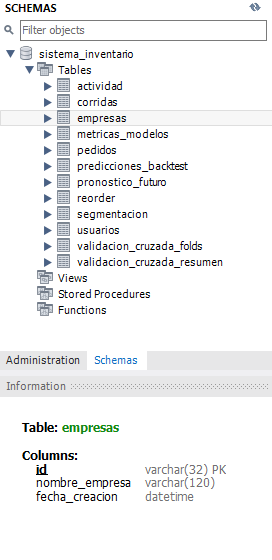
\includegraphics[height=0.35\textheight]{templatefigures/mysql_workbench_empresas}
    \caption{Estructura de la tabla \texttt{empresas} vista desde MySQL Workbench, conectado a la base de datos local.}
    \label{fig:mysql_workbench_empresas}
\end{figure}

La tabla \texttt{empresas} existe en la base de datos con las columnas descritas anteriormente: un identificador de tipo \texttt{varchar(32)} como clave primaria, el nombre de la empresa, y la fecha de creación del registro.

\begin{figure}[H]
    \centering
    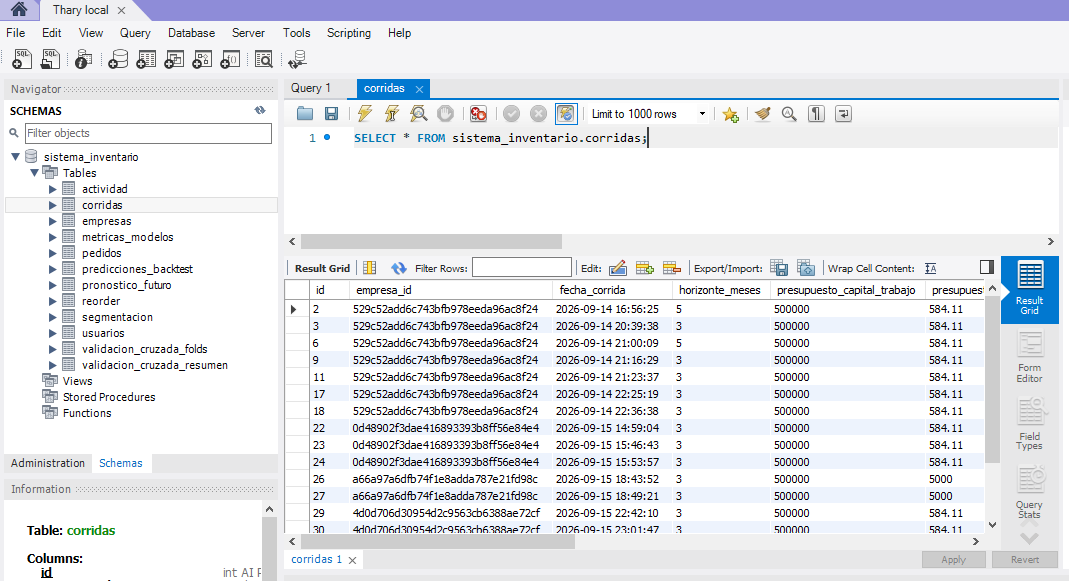
\includegraphics[height=0.3\textheight]{templatefigures/mysql_workbench_corridas}
    \caption{Consulta sobre la tabla \texttt{corridas} en MySQL Workbench, mostrando el esquema completo de 12 tablas y el historial acumulado de corridas.}
    \label{fig:mysql_workbench_corridas}
\end{figure}

La Fig. \ref{fig:mysql_workbench_corridas} muestra la confirmación de que cada procesamiento de archivo genera una fila nueva en \texttt{corridas} sin eliminar las anteriores. Existen múltiples filas asociadas a una misma empresa, correspondientes a distintas corridas realizadas en distintasfechas y horas.
